% CS466 Deep Learning - Term Project Final Report
% Compile with pdfLaTeX from this folder:  latexmk -pdf report.tex
% Figures are read from ../../figures (made by scripts/make_figures.py and scripts/qualitative.py).

\documentclass[11pt]{article}

\usepackage[utf8]{inputenc}
\usepackage[T1]{fontenc}
\usepackage{lmodern}
\usepackage[margin=0.9in]{geometry}
\usepackage{amsmath,amssymb}
\usepackage{booktabs}
\usepackage{graphicx}
\usepackage{enumitem}
\usepackage{caption}
\usepackage[hidelinks]{hyperref}

\graphicspath{{../../figures/}}
\setlist{itemsep=1pt, topsep=3pt}
\captionsetup{font=small, labelfont=bf}
\newcommand{\best}[1]{\textbf{#1}}

\title{\textbf{Small and Fast Depth Estimation with Few Labels\\by Learning from a Big Model}\\[4pt]
\large CS466 Deep Learning, Fall 2026 --- Term Project Final Report}
\author{Oğuz Kağan Göçmez\\
\small Özyeğin University\\
\small \texttt{kagan.gocmez@ozu.edu.tr}}
\date{December 2026}

\begin{document}
\maketitle

%--------------------------------------------------------------------
\begin{abstract}
\noindent
Monocular depth estimation needs dense depth labels, which are expensive to collect, and the most
accurate models are too large for small devices. I study whether a small student network
(1--4M parameters) can learn metric depth from a few labeled images plus a large foundation
model, Depth Anything V2 Small (24.8M parameters), that gives relative depth on every image.
The student is trained with a scale-invariant loss on the labeled images and a
scale-and-shift-invariant loss against the teacher on all images. On NYU Depth V2 I vary the
share of labeled training images from 1\% to 100\% and compare against the same student trained
on the labels only. With 1\% of the labels (462 images) the teacher lowers the test AbsRel of a
3.15M-parameter student by 13\% (0.195 to 0.169, three seeds). The gain holds for other labeled
subsets, other student sizes and together with the usual regularizers. It shrinks as labels are
added: with a constant teacher weight the student becomes worse than the label-only baseline from
25\% labels on. Fading the teacher out over the second half of training and keeping it off the
labeled images removes this harm and keeps a small gain at 5\% ($-5$\%) and 25\% ($-2$\%). An error
analysis shows that the teacher mainly improves the shape of the depth map, while the metric
scale still comes from the labels. The final student is 8$\times$ smaller and 5$\times$ faster
than the teacher (8.5\,ms on a laptop GPU) and with all labels reaches an AbsRel of 0.150 and
$\delta_1$ of 0.794 on the NYU test set.
\end{abstract}

%--------------------------------------------------------------------
\section{Introduction}

A robot or a phone that wants to know how far away things are can use a depth sensor, but a
normal camera is cheaper and almost always there. \emph{Monocular depth estimation} predicts a
depth value for every pixel of a single RGB image~\cite{eigen2014}. Two problems make this hard in
practice. First, the strongest recent models, such as Depth Anything V2~\cite{yang2024dav2}, are
large vision transformers that are too slow for small devices. Second, training a model that
outputs depth in meters needs real depth maps, and these must be recorded with a depth sensor for
every scene.

\emph{Knowledge distillation}~\cite{hinton2015} addresses both problems at once: a large
\emph{teacher} labels images for free and a small \emph{student} learns from it. For depth there
is a catch. Foundation models like Depth Anything predict \emph{relative} inverse depth, which is
correct only up to an unknown scale and shift per image, so they cannot teach metric depth on
their own. The student therefore needs both signals: the few real depth maps for the scale, and
the teacher for everything else.

This project studies \textbf{when the teacher helps a very small student and when it does not}.
I keep the real depth for only part of the NYU Depth V2~\cite{silberman2012} training images
(1\%, 5\%, 25\% or 100\%), train the same student with and without the teacher, and evaluate all
models on the standard test set only once, at the end. My main findings are:
\begin{itemize}
  \item With very few labels the teacher clearly helps: $-13\%$ test AbsRel at 1\% labels, on
        every labeled subset, student size and regularizer I tried.
  \item The gain shrinks as labels are added, and with a constant teacher weight the teacher
        becomes harmful from 25\% on. Two simple changes, a teacher weight that decays to zero
        and no teacher loss on labeled images, remove the harm.
  \item The teacher improves the \emph{shape} of the depth map much more than its \emph{scale};
        the scale error is the same with and without it.
  \item The 3.15M student needs 144$\times$ fewer FLOPs than the teacher and runs in 8.5\,ms.
\end{itemize}
All code, run logs and results are public.\footnote{\url{https://github.com/oguz-kagan-gocmez-edu/knowledge-distillation-depth}}

%--------------------------------------------------------------------
\section{Related Work}

\paragraph{Supervised monocular depth.} Eigen et al.~\cite{eigen2014} trained the first deep
network for single-image depth and introduced the scale-invariant log loss that I use for the
labeled images. Later work improved accuracy on NYU with deeper encoders and better decoders:
Laina et al.~\cite{laina2016} (fully convolutional ResNet-50), DORN~\cite{fu2018} (depth as
ordinal regression) and BTS~\cite{lee2019} (local planar guidance). These models are large and use
all the labels.

\paragraph{Lightweight depth.} FastDepth~\cite{wofk2019} showed that a MobileNet encoder with a
light decoder runs in real time on embedded hardware. My student follows the same design, with a
MobileNetV3~\cite{howard2019} or EfficientNet-B0~\cite{tan2019} encoder. Unlike FastDepth, it is
trained with few labels and a teacher.

\paragraph{Relative depth and foundation models.} MiDaS~\cite{ranftl2022} trained on many
datasets with different scales by using a scale-and-shift-invariant loss and a gradient-matching
loss; I use both for the teacher term. Depth Anything~\cite{yang2024dav1} and Depth Anything
V2~\cite{yang2024dav2} scaled this up with millions of pseudo-labeled images and are today among
the best zero-shot relative depth models. Depth Anything itself is trained by distillation: a
large teacher labels unlabeled images and the student learns them under strong perturbations.

\paragraph{Distillation for depth.} Wang et al.~\cite{wang2021kd} distilled a large depth network
into a mobile one, with all labels available. ZipDepth~\cite{tosi2026zipdepth} recently distilled
a foundation model into a lightweight zero-shot model using 14.1M images and many GPUs. My work
looks at the other end: a very small student, one dataset, a single GPU and, most importantly,
only a few labeled images. I also study a question these works do not ask directly: how the value
of the teacher changes with the number of labels.

\paragraph{Semi-supervised learning.} Training on labeled images together with targets from a
teacher on unlabeled images is a form of pseudo-labeling, as in Noisy Student~\cite{xie2020} or
Mean Teacher~\cite{tarvainen2017}. The difference here is that the teacher is fixed, much larger
than the student, and its targets are only relative.

%--------------------------------------------------------------------
\section{Data}

\paragraph{Dataset.} NYU Depth V2~\cite{silberman2012} contains indoor scenes recorded with a
Microsoft Kinect. I use the widely used DenseDepth copy~\cite{alhashim2018}: 50,688 training
images from 249 rooms with filled depth maps (no missing pixels), and the standard 654-image test
set (Eigen split) from other rooms. All images are $640\times480$; depth is stored in millimeters
and converted to meters.

\paragraph{Validation split by room.} Consecutive frames from the same room are almost identical,
so a random validation split would measure memorization. I hold out 25 whole rooms (10\%) for
validation and use 1,000 images from them. The remaining 46,248 images from 224 rooms form the
training \emph{pool}. All choices in this report (training length, loss weights, teacher schedule)
were made on this validation set. The 654 test images were used once, after all training runs had
ended.\footnote{Two groups of extra seeds (Section~\ref{sec:gtmask}) were trained after this
evaluation. Their settings had been fixed before it; they only add seeds and were evaluated on the
test set separately.}

\paragraph{Label budgets.} To simulate few labels, I keep the real depth for a random subset of
the pool: 462 (1\%), 2,312 (5\%), 11,562 (25\%) or all 46,248 (100\%) images. The rest are treated
as unlabeled. The subset depends on a fixed seed, so all recipes at a budget see the same labeled
images; two more random 1\% subsets check that the results do not depend on the choice.

\paragraph{Preprocessing.} Images and depth maps are resized to $256\times192$ for training. The
teacher is run once on every pool and validation image at its native resolution ($686\times518$
for a $640\times480$ image) and its output, relative inverse depth, is stored at $256\times192$
in half precision ($\sim$5\,GB). Training therefore never runs the teacher. The only augmentation
in the main runs is a random horizontal flip, applied to the image, the depth and the teacher
output together.

%--------------------------------------------------------------------
\section{Methods}

\subsection{Teacher and student}

\paragraph{Teacher.} Depth Anything V2 Small~\cite{yang2024dav2} (24.8M parameters, a DINOv2
ViT-S encoder with a DPT decoder), loaded through Hugging Face Transformers~\cite{wolf2020}. It is
used without any fine-tuning.

\paragraph{Student.} An encoder--decoder network in the style of FastDepth~\cite{wofk2019},
written for this project in PyTorch~\cite{paszke2019}. The encoder is an ImageNet-pretrained
backbone from torchvision~\cite{paszke2019}. The decoder takes the encoder features at strides 32,
16, 8, 4 and 2: a $1\times1$ bottleneck, then four steps of bilinear upsampling, concatenation with
the skip feature and a depthwise-separable convolution block, and finally a small head. A sigmoid
maps the output to $[0.001, 10]$ meters. Three sizes are used:

\begin{center}\small
\begin{tabular}{@{}lllr@{}}
\toprule
Size & Encoder & Decoder width & Parameters \\
\midrule
tiny  & MobileNetV3-Small~\cite{howard2019} & 16 & 0.98M \\
small (default) & MobileNetV3-Large~\cite{howard2019} & 32 & 3.15M \\
base  & EfficientNet-B0~\cite{tan2019} & 32 & 4.23M \\
\bottomrule
\end{tabular}
\end{center}

\subsection{Losses}

The training loss for a batch is
\begin{equation}
  \mathcal{L} = \mathcal{L}_{\text{gt}}
  + w(t)\,\big(\lambda_t\,\mathcal{L}_{\text{teacher}} + \lambda_e\,\mathcal{L}_{\text{edge}}\big),
  \qquad \lambda_t = 1,\ \lambda_e = 0.5 .
\end{equation}

\paragraph{Real depth.} $\mathcal{L}_{\text{gt}}$ is the scale-invariant log loss~\cite{eigen2014}
over the valid pixels of the labeled images in the batch, with $d_i = \log \hat{y}_i - \log y_i$:
\begin{equation}
  \mathcal{L}_{\text{gt}} = \sqrt{\tfrac{1}{n}\textstyle\sum_i d_i^2 - 0.85\,\big(\tfrac{1}{n}\sum_i d_i\big)^2}.
\end{equation}
It is the only term that sees metric depth, so it is the only source of the scale.

\paragraph{Teacher.} The teacher gives inverse depth $t$ with an unknown scale and shift. I convert
the student's depth to inverse depth, $p = 1/\hat{y}$, and normalize both maps per image by their
median and mean absolute deviation, as in MiDaS~\cite{ranftl2022}:
\begin{equation}
  \tilde{x} = \frac{x - \operatorname{med}(x)}{\tfrac{1}{n}\sum_i |x_i - \operatorname{med}(x)|},
  \qquad
  \mathcal{L}_{\text{teacher}} = \tfrac{1}{n}\textstyle\sum_i |\tilde{p}_i - \tilde{t}_i| .
\end{equation}
This loss never uses real depth, so it works on unlabeled images, and it cannot conflict with the
scale learned from the labels.

\paragraph{Edges.} $\mathcal{L}_{\text{edge}}$ is the multi-scale gradient-matching loss of
MiDaS~\cite{ranftl2022}: the mean absolute horizontal and vertical gradient of the residual
$\tilde{p} - \tilde{t}$, at four scales. It asks the student to copy the teacher's sharp object
borders.

\paragraph{Teacher schedule.} The teacher weight $w(t)$ grows linearly from 0 to 1 over the first
30\% of training, so the student first learns the metric scale from the labels. In the
\emph{teacher decay} variant it then falls linearly back to 0 over the second half of training
(Section~\ref{sec:decay}).

\subsection{Recipes}

Every batch has 8 images. The recipes differ in which images are used and which loss terms are
on:

\begin{center}\small
\begin{tabular}{@{}lll@{}}
\toprule
ID & Batch & Loss \\
\midrule
E1 \texttt{gt} & 8 labeled images & $\mathcal{L}_{\text{gt}}$ (baseline, no teacher) \\
E2 \texttt{gt\_t} & 8 labeled images & $\mathcal{L}_{\text{gt}} + \mathcal{L}_{\text{teacher}}$ \\
E3 \texttt{semi} & 4 labeled + 4 from the whole pool & $\mathcal{L}_{\text{gt}}$ on labeled, $\mathcal{L}_{\text{teacher}}$ on all 8 \\
E4 \texttt{semi\_edge} & as E3 & E3 + $\mathcal{L}_{\text{edge}}$ (full recipe) \\
\bottomrule
\end{tabular}
\end{center}

E2 tests whether the teacher helps as an extra signal on the same images; E3 adds the unlabeled
images; E4 adds the edge term. E1 is the fair baseline: the same network, data, schedule and
labeled images, only without the teacher.

\subsection{Training and evaluation}

All runs use AdamW~\cite{loshchilov2019} (learning rate $5\cdot10^{-4}$, weight decay $10^{-4}$),
a one-cycle schedule~\cite{smith2019} with 10\% warm-up, gradient clipping at 1.0 and
24,000 steps. Every 3,000 steps the model is evaluated on the 1,000 validation images; the
checkpoint with the lowest validation AbsRel (``best'') is kept together with the final one.
A run takes about 20 minutes on a Colab L4 GPU. In total I trained 88 runs ($\sim$32 GPU hours),
with automatic resumption from checkpoints after disconnects.

For the test set the prediction is upsampled from $256\times192$ to $640\times480$ and scored
inside the Eigen crop on pixels between 0.001 and 10\,m, the usual NYU protocol. I report
AbsRel, RMSE (per image, then averaged) and $\delta_1$ (share of pixels with
$\max(\hat{y}/y, y/\hat{y}) < 1.25$) on the raw metric predictions, without any per-image
scaling. Validation numbers are computed at $256\times192$ without the crop.

\paragraph{Alternatives I considered.} I did not fine-tune the teacher to metric depth, because
that would need the same labels the student lacks, and its outputs would then share the student's
errors. I also did not use feature distillation: the teacher (a ViT) and the student (a CNN) have
very different features, and storing teacher features for 46k images would cost far more than
the 5\,GB of depth maps. Matching outputs keeps the teacher a black box that can be swapped.

%--------------------------------------------------------------------
\section{Experiments}

\subsection{References}

Two references bound the possible results. A constant prediction (the median depth of the labeled
images) gets a validation AbsRel of 0.402. The teacher, after its scale and shift are fitted to the
real depth \emph{of each test image}, gets a test AbsRel of 0.062, RMSE 0.297 and $\delta_1$ 0.956,
close to the 0.053 that Depth Anything V2 reports for this model with the same kind of
alignment~\cite{yang2024dav2}. This is an optimistic upper bound: no student can fit its output to
real depth it does not have. On validation the same reference gives 0.110, most likely because the
cached teacher output is at $256\times192$, there is no crop and the held-out rooms are harder.

\subsection{Preliminary result: with all labels the teacher does not help}

Before the main study I ran a short feasibility test on 2,000 fully labeled images: the student
trained with the teacher (AbsRel 0.204) was no better than without it (0.202). The NYU training
depth maps are already filled, so with full labels the teacher repeats information the student has.
This result moved the project to the few-label setting.

\subsection{Main result: the effect of the teacher by label budget}

Figure~\ref{fig:budget} and Table~\ref{tab:test} show the main comparison on the test set.

\begin{figure}[t]
  \centering
  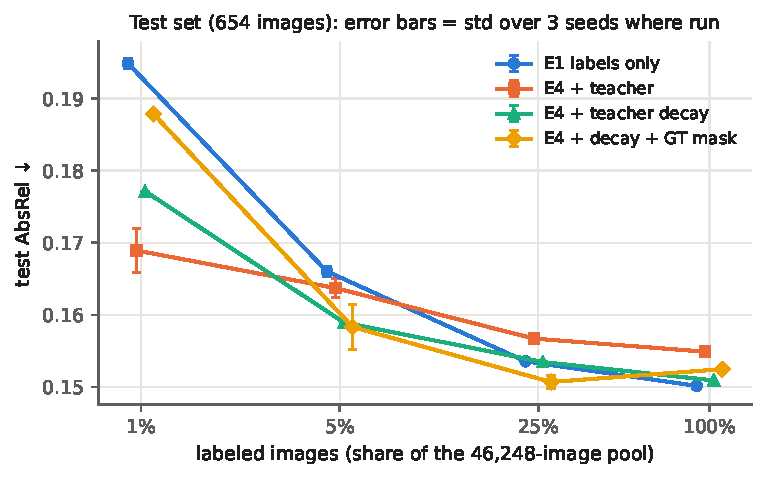
\includegraphics[width=0.66\linewidth]{test_budget.pdf}
  \caption{Test AbsRel of the 3.15M student against the share of labeled images. Error bars show
  the standard deviation over three seeds where three were run.}
  \label{fig:budget}
\end{figure}

\begin{table}[t]
\centering\small
\begin{tabular}{@{}lcccc@{}}
\toprule
Labeled & E1 (labels only) & E4 & E4 + decay & E4 + decay + GT mask \\
\midrule
1\% (462)       & 0.195 $\pm$ 0.001 & \best{0.169 $\pm$ 0.003} & 0.177 & 0.188 \\
5\% (2,312)     & 0.166 $\pm$ 0.001 & 0.164 $\pm$ 0.001 & 0.159 & \best{0.158 $\pm$ 0.003} \\
25\% (11,562)   & 0.154 $\pm$ 0.000 & 0.157 & 0.153 & \best{0.151 $\pm$ 0.001} \\
100\% (46,248)  & \best{0.150} & 0.155 & 0.151 & 0.152 \\
\bottomrule
\end{tabular}
\caption{Test AbsRel ($\downarrow$) of the small student, best-on-validation checkpoints. Values
with $\pm$ are the mean and standard deviation over three seeds, the others one seed. The decay and
GT-mask variants are explained in Sections~\ref{sec:decay} and~\ref{sec:gtmask}.}
\label{tab:test}
\end{table}

\paragraph{Few labels.} At 1\% the teacher lowers AbsRel from 0.195 to 0.169 ($-13\%$), RMSE from
0.646 to 0.580 and raises $\delta_1$ from 0.698 to 0.754. The difference is about nine times the
larger standard deviation over seeds. In raw AbsRel, 1\% labels with the teacher are about as good
as 5\% labels without it (0.169 vs.\ 0.166).

\paragraph{More labels.} The gain shrinks quickly. At 5\% the plain E4 is only 1\% better than E1,
and at 25\% and 100\% it is 2--3\% \emph{worse}. With enough labels the relative teacher target
starts to compete with the real depth.

\subsection{Why the teacher helps: memorization at 1\%}

Figure~\ref{fig:curves} shows the validation curves. At 1\%, E1 goes over its 462 images more
than a thousand times in a long run (Figure~\ref{fig:epochs}). Its training loss keeps falling
(SILog $\approx 0.07$) while its validation error stops improving after about 100 passes: it
memorizes the labeled images. With the teacher the training SILog stays near 0.16 and the
validation error is lower at every point. The teacher acts as a strong regularizer that keeps the
student from fitting its few labels exactly, and at the same time shows it many more scenes.

\begin{figure}[t]
  \centering
  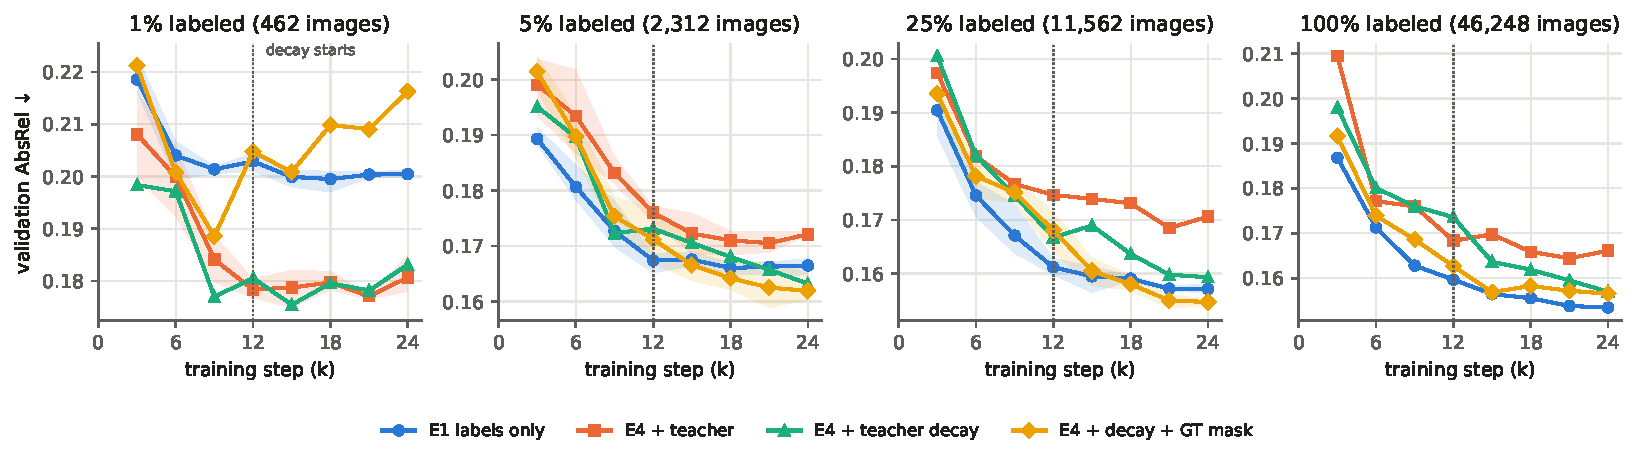
\includegraphics[width=\linewidth]{val_curves.pdf}
  \caption{Validation AbsRel during training (mean over seeds, band from minimum to maximum).
  The dotted line marks where the teacher decay starts.}
  \label{fig:curves}
\end{figure}

\begin{figure}[t]
  \centering
  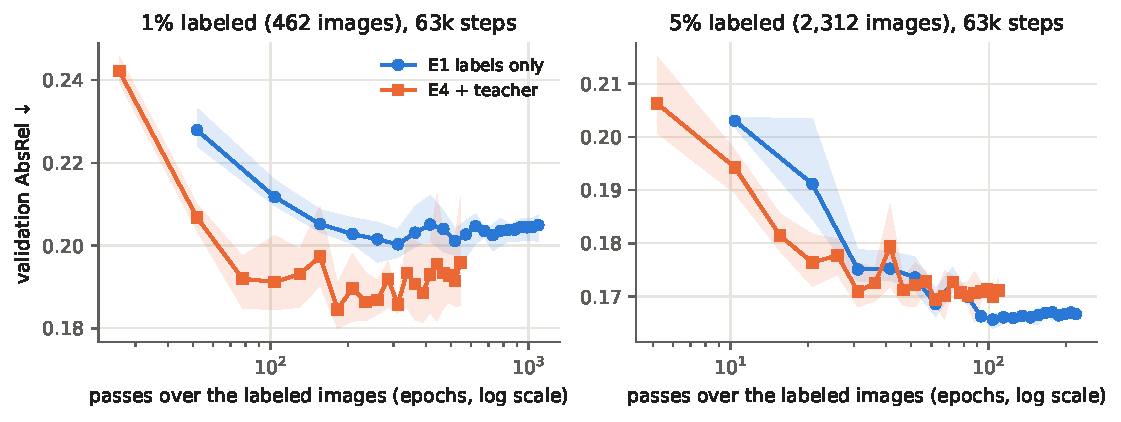
\includegraphics[width=0.85\linewidth]{epochs.pdf}
  \caption{Validation AbsRel against passes over the labeled images, for 63k-step runs (three
  seeds). E1 sees 8 labeled images per step, E4 four.}
  \label{fig:epochs}
\end{figure}

\paragraph{Training length.} My original plan used 63k steps. At 1\% E4 then reached its best
validation error in the middle of training and degraded later on two of three seeds (final AbsRel
0.196 $\pm$ 0.011), while its predicted scale drifted. With 24k steps this no longer happened and
the best results were the same, so all later runs use 24k steps.

\subsection{Ablation: which part of the teacher helps}

\begin{table}[t]
\centering\small
\begin{tabular}{@{}lcccc@{}}
\toprule
& \multicolumn{2}{c}{Validation} & \multicolumn{2}{c}{Test} \\
\cmidrule(lr){2-3}\cmidrule(lr){4-5}
Recipe & 1\% & 5\% & 1\% & 5\% \\
\midrule
E1 labels only                          & 0.199 & 0.166 & 0.196 & 0.167 \\
E2 + teacher on labeled images          & 0.195 & 0.174 & 0.191 & 0.164 \\
E3 + teacher on all images              & 0.177 & 0.172 & \best{0.167} & \best{0.157} \\
E4 + teacher on all images + edge loss  & \best{0.176} & 0.170 & \best{0.166} & 0.165 \\
\bottomrule
\end{tabular}
\caption{AbsRel ($\downarrow$) of the four recipes. E2 and E3 have one seed; for E1 and E4 the
validation columns are three-seed means and the test columns seed 0, so all test numbers come from
the same seed.}
\label{tab:ablation}
\end{table}

Table~\ref{tab:ablation} separates the parts of the recipe. Adding the teacher only on the labeled
images (E2) changes little. The gain comes from the teacher's targets on the \emph{unlabeled}
images (E3). The edge loss (E4) adds nothing measurable; on the test set E3 is even slightly
better at 5\%. The teacher's value is therefore not a better signal on the same images but
supervision on images that have no labels.

\subsection{Robustness of the 1\% result}

Figure~\ref{fig:checks} repeats the 1\% comparison under eight changes. The teacher lowers test
AbsRel in every case: on two other random labeled subsets ($-12\%$, $-13\%$), with the 1M and 4M
students ($-7\%$, $-4\%$), with 63k steps ($-9\%$) and together with the usual regularizers.

\begin{figure}[t]
  \centering
  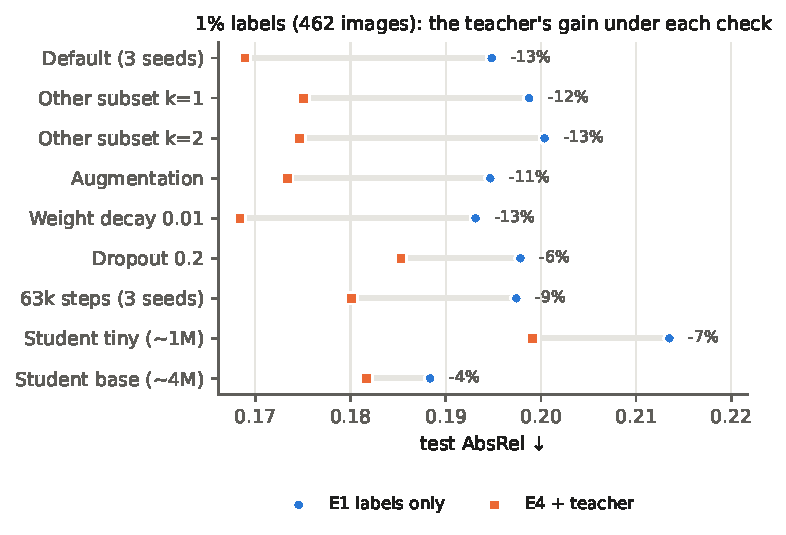
\includegraphics[width=0.62\linewidth]{test_checks_1.pdf}
  \caption{Test AbsRel at 1\% labels, E1 and E4, under each check (seed 0 unless noted).}
  \label{fig:checks}
\end{figure}

\paragraph{Regularizers vs.\ the teacher.} Since E1 memorizes at 1\%, I tried the usual remedies,
one at a time, on both recipes (validation AbsRel, E1 / E4): random zoom-in crops with color
jitter, 0.195 / 0.173; weight decay 0.01 instead of $10^{-4}$, 0.198 / 0.173; and channel dropout
0.2, 0.204 / 0.192. Augmentation helps a little (about 2\%), stronger weight decay does nothing
(the network is mostly batch-normalized, so the scale of its weights barely matters), and dropout
makes E4 underfit. None of them comes close to the teacher's gain, and the teacher's gain stays the
same with augmentation or weight decay, so the two add up.

\subsection{Teacher decay}
\label{sec:decay}

The validation curves (Figure~\ref{fig:curves}) suggested that with many labels the teacher holds
the student back late in training: E4's training SILog stays near 0.18, while E1 keeps improving.
I therefore let the teacher weight fall to zero over the second half of training. On validation
this removed most of the harm at 25\% and 100\% (E4 0.168 $\to$ 0.159, 0.164 $\to$ 0.157) and gave
the best 5\% result so far (0.163), but at 1\% the student started to memorize again once the
teacher was gone (training SILog 0.162 $\to$ 0.098, validation 0.175 $\to$ 0.183 at the last step).
On the test set the decay reaches the level of E1 at 25\% and 100\% (Table~\ref{tab:test}).
After the test evaluation I also checked, on validation only, whether the late overfitting at 1\%
comes from removing the teacher completely or only from lowering its weight: with the weight
falling to 0.25 instead of 0, training SILog ends at 0.111 and validation stays flat to the last
step (0.177), but the best checkpoint is unchanged (0.176). At 5\% this lands between a constant
teacher and the full decay (0.167 vs.\ 0.170 and 0.163). All three differences are within the noise
of one seed, so I kept the full decay.

\subsection{Keeping the teacher off the labeled images}
\label{sec:gtmask}

In E3/E4 four images of each batch are drawn from the whole pool. In my first implementation the
real depth of these images was ignored even when they were labeled, and the teacher loss was
applied to every image. So at 100\% labels E4 saw only 4 labeled images per step against 8 for E1,
and the teacher pulled against the real depth on every labeled pixel. I added an option that uses
the real depth of every labeled image in the batch and turns the teacher off on them (``GT mask''),
so the teacher only supervises images without labels. At 100\% every image is labeled, so this run
has no teacher at all and should behave like E1: its training loss indeed matched E1 to the third
decimal at every evaluation, but its validation AbsRel ended at 0.157 against 0.153, only because
the batches came in another order. This sanity check showed that one seed can move AbsRel by
$\sim$0.004 with many labels, so I ran two more seeds of GT mask at 5\% and 25\%, and of E1 at
25\%.

With three seeds GT mask is the best setting at 5\% (test 0.158 $\pm$ 0.003 vs.\ 0.166 for E1,
all three seeds below E1) and at 25\% (0.151 $\pm$ 0.001 vs.\ 0.154). At 1\%, however, it is much
worse (0.188): the teacher on the labeled images was what stopped the student from memorizing
them. The best teacher setting therefore depends on the label budget, and no single recipe wins
everywhere.

\subsection{Larger teacher and larger student}

After the test, with settings fixed beforehand and on validation only, I changed only the teacher or
only the student (seed 0). With Depth Anything V2 Base (97.5M) and Large (335M) as teachers, E4
gets 0.176 and 0.178 at 1\% and 0.169 and 0.166 at 5\%, against 0.176 and 0.170 with Small: all
within seed noise. This holds although the Base teacher is itself better than Small (aligned
reference 0.106 vs.\ 0.110); at the cached $256\times192$ input the Large teacher is worse (0.121),
which may be due to the low resolution, but I did not test this. The base student (EfficientNet-B0,
4.23M) gets 0.152 at 25\% with decay and GT mask, against $0.155\pm0.001$ for the small student,
and 0.153 at 100\% with E1, the same as the small student. So neither a 13$\times$ larger teacher nor a
35\% larger student closes the gap to the teacher reference: the gain comes from the unlabeled
images, not from model size.

\subsection{Where the teacher helps: shape vs.\ scale}

\begin{figure}[t]
  \centering
  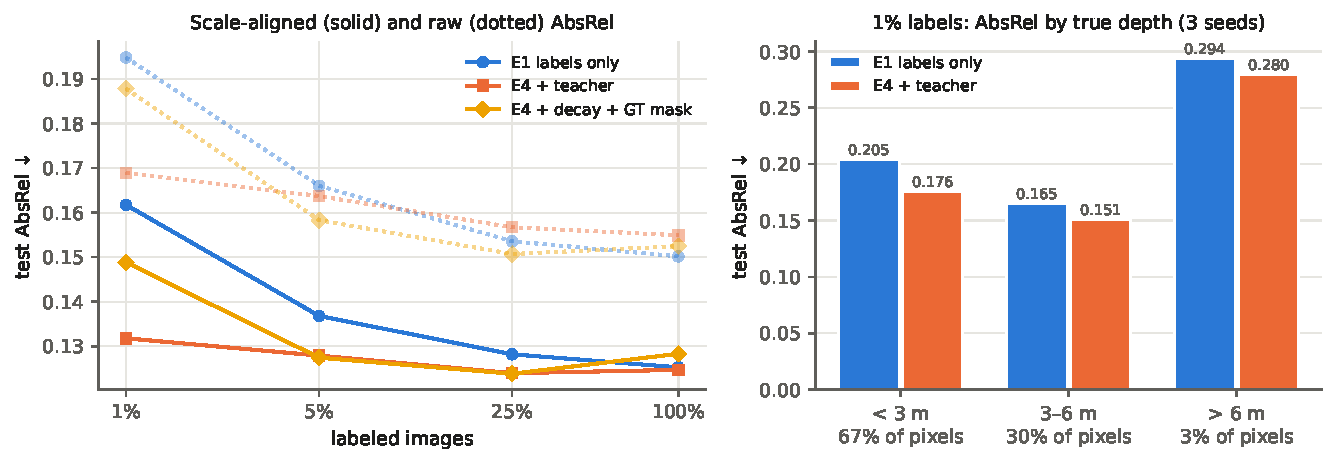
\includegraphics[width=\linewidth]{test_errors.pdf}
  \caption{Left: test AbsRel after scaling each prediction by $\operatorname{med}(y)/\operatorname{med}(\hat{y})$
  (solid) and without (dotted). Right: test AbsRel by true depth at 1\% labels (three seeds).}
  \label{fig:errors}
\end{figure}

To see \emph{what} the teacher improves, I also score every prediction after scaling it by the
ratio of the medians of real and predicted depth, which removes its overall scale
(Figure~\ref{fig:errors}, left). At 1\% the teacher lowers this scale-free error by 19\%
(0.162 $\to$ 0.132), more than the raw error (13\%). The part of the error caused by the scale
(raw minus aligned, $\sim$0.03--0.04) is about the same with and without the teacher. In shape,
1\% labels with the teacher (0.132) are close to 25\% labels without it (0.128). At 25\% the
teacher still gives a slightly better shape (0.124 vs.\ 0.128) but a worse raw error: what the
constant-weight E4 loses with many labels is the scale. This matches the design of the losses:
the teacher term is scale-free by construction, so the metric scale can only come from the labels.

By distance (Figure~\ref{fig:errors}, right), the gain at 1\% is largest for near pixels
($<3$\,m, 67\% of all pixels: 0.205 $\to$ 0.176) and smallest beyond 6\,m (0.294 $\to$ 0.280). From
5\% on E4 is even worse than E1 beyond 6\,m (0.289 vs.\ 0.267). The teacher loss is computed on
inverse depth, where far distances are compressed, and the teacher itself is weakest there (aligned
AbsRel 0.17 beyond 6\,m against 0.06 below 3\,m).

\subsection{Qualitative results and failure cases}

Figure~\ref{fig:qual} shows four test images spaced evenly over the test set (not selected by
result). In the first row the label-only student gets the layout of the room wrong (AbsRel 0.235),
while the student with the teacher follows the walls and shelves (0.140), close to the student
trained on all labels (0.124). Object outlines such as chairs are much sharper with the teacher. The
third row is a typical failure: both 1\% students place the back wall too far and get the overall
scale wrong (AbsRel 0.43 and 0.47). The teacher cannot correct this, since it only provides relative
depth.

\begin{figure}[t]
  \centering
  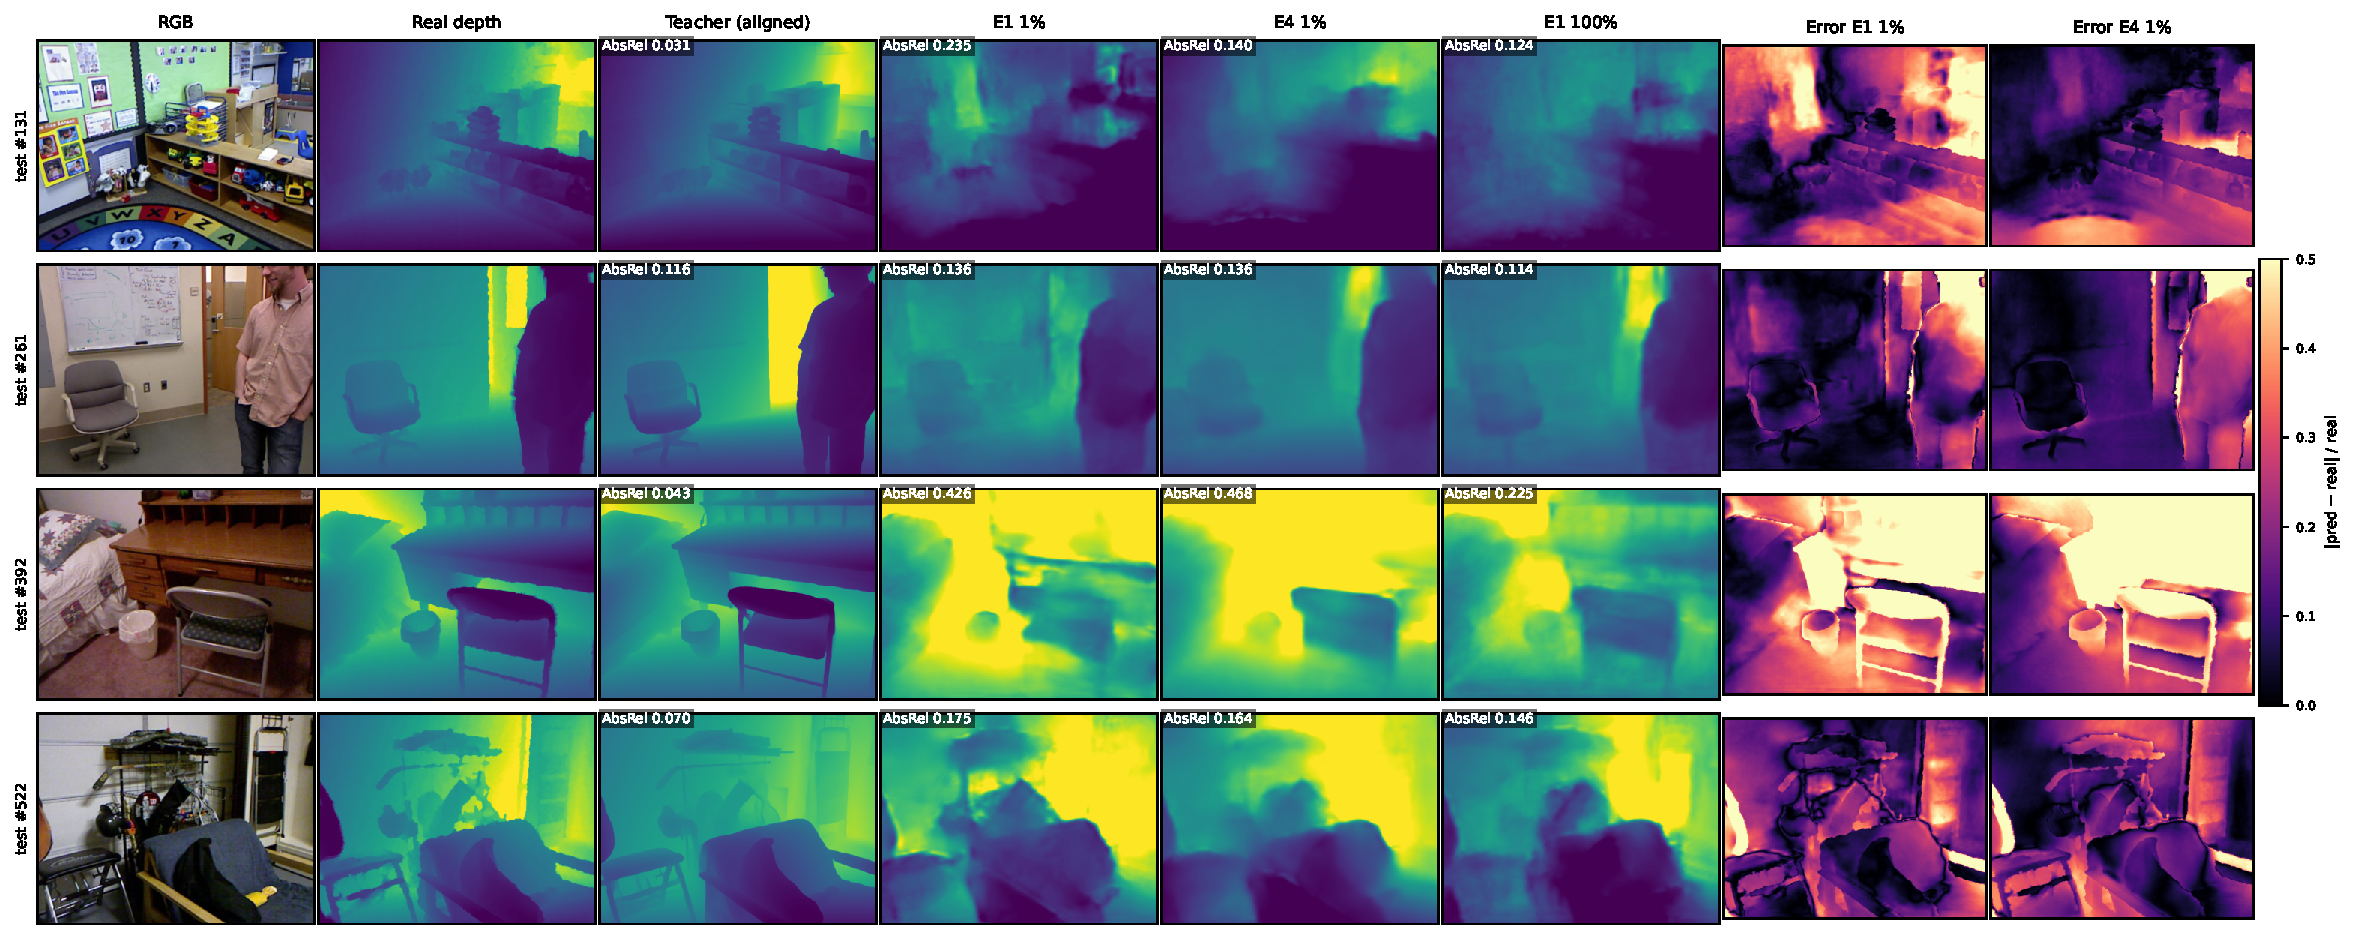
\includegraphics[width=\linewidth]{qualitative.pdf}
  \caption{Test examples. Columns: input, real depth, teacher aligned per image to the real depth,
  students trained with 1\% labels without (E1) and with (E4) the teacher, E1 with all labels, and
  the per-pixel relative error of the two 1\% students. Depth maps of a row share one color
  scale.}
  \label{fig:qual}
\end{figure}

\subsection{Size and speed}

\begin{table}[t]
\centering\small
\begin{tabular}{@{}llrrr@{}}
\toprule
Model & Input & Parameters & GFLOPs & Latency \\
\midrule
Teacher, Depth Anything V2 Small & $686\times518$ & 24.8M & 106.8 & 45.1\,ms \\
Teacher at the students' input size & $252\times196$ & 24.8M & 14.9 & 10.0\,ms \\
Student tiny & $256\times192$ & 0.98M & 0.21 & 7.0\,ms \\
\best{Student small} & $256\times192$ & \best{3.15M} & \best{0.74} & \best{8.5\,ms} \\
Student base & $256\times192$ & 4.23M & 1.08 & 10.3\,ms \\
\bottomrule
\end{tabular}
\caption{Size and speed, batch 1, model only, median of 50 passes on an Apple M4 Pro GPU.}
\label{tab:speed}
\end{table}

Table~\ref{tab:speed} compares the models. The small student has 8$\times$ fewer parameters and
needs 144$\times$ fewer FLOPs than the teacher at the input the teacher actually uses, and it runs
5$\times$ faster. The speed-up is much smaller than the FLOP ratio because at batch 1 the GPU time
of such small networks is dominated by kernel launch overhead. I also measured on the CPU, but the
macOS build of PyTorch has no fast kernel for depthwise convolutions, so there the students were
not faster than the teacher at the same input size; a deployment would need an optimized runtime.

\subsection{Comparison with published models}

\begin{table}[t]
\centering\small
\begin{tabular}{@{}llccc@{}}
\toprule
Model & Labels & AbsRel $\downarrow$ & RMSE $\downarrow$ & $\delta_1 \uparrow$ \\
\midrule
Eigen \& Fergus~\cite{eigen2015} & all & 0.158 & 0.641 & 0.769 \\
FastDepth~\cite{wofk2019} (MobileNet) & all & -- & 0.604 & 0.771 \\
\best{Ours, small student (E1)} & 100\% & \best{0.150} & \best{0.526} & \best{0.794} \\
\best{Ours, small student (E4)} & 1\% & 0.169 & 0.580 & 0.754 \\
Laina et al.~\cite{laina2016} (ResNet-50) & all & 0.127 & 0.573 & 0.811 \\
DORN~\cite{fu2018} & all & 0.115 & 0.509 & 0.828 \\
BTS~\cite{lee2019} & all & 0.110 & 0.392 & 0.885 \\
\bottomrule
\end{tabular}
\caption{NYU Depth V2 test set. Not a strict comparison: resolution, training data and the way
RMSE is averaged differ (mine is the mean of per-image RMSE).}
\label{tab:published}
\end{table}

Table~\ref{tab:published} places the student among published results on the same test set. With
all labels it is in the range of full-size models from 2015--2016, ahead of FastDepth, which has a
similar size. With only 1\% of the labels and the teacher it is still close to Eigen \&
Fergus~\cite{eigen2015}, which used all labels. Recent large models remain far more accurate.

%--------------------------------------------------------------------
\section{Discussion and Limitations}

\paragraph{Noise.} Most settings beyond the main comparison have a single seed. The 100\% sanity
check showed that one seed can move AbsRel by $\sim$0.004 (2.5\%) with many labels, while with few
labels the seed spread was smaller ($\pm$0.001--0.003). I therefore only call differences larger
than about 3\% clear, and ran three seeds for every claim that depends on smaller differences.

\paragraph{Selection on validation.} The test set was used once, but the recipes compared on it were
chosen from many validation runs. The best setting per budget in Table~\ref{tab:test} is thus
slightly optimistic; the plain E1 vs.\ E4 comparison, fixed in the proposal, is not.

\paragraph{One dataset and one teacher.} All results are on indoor NYU images, and the main results
use a single teacher (the larger teachers were tried on validation only, at one input size).
The conclusions about scale may change outdoors, where depth ranges are larger and the teacher's
weakness at far distances matters more.

%--------------------------------------------------------------------
\section{Conclusion}

A very small depth network can learn a great deal from a large relative-depth model when real depth
is scarce. With 1\% of the labels, a 3.15M-parameter student trained with Depth Anything V2 Small
nearly reaches the accuracy of the same student trained on five times more labels, and the gain is stable
across labeled subsets, student sizes and regularizers. Its source is clear: the teacher supervises
the unlabeled images and keeps the student from memorizing its few labels, and it mostly improves
the shape of the depth map, while the metric scale must come from the labels. The value of the
teacher falls as labels are added, and a constant teacher weight eventually hurts; letting the
teacher fade out and keeping it off labeled images avoids this.

\paragraph{Future work.} Three directions follow from the analysis. (1) A budget-aware schedule
that keeps the teacher on labeled images when labels are very few and turns it off when they are
many, instead of choosing one recipe by hand. (2) Better scale: since the scale comes only from the
labels, a scale estimated from few labels per scene, or the teacher's own metric variant, could
target the error that the teacher cannot fix. (3) A teacher loss in depth rather than inverse depth,
or weighted toward far pixels, to remove the loss beyond 6\,m. Methods that I found in the
literature but did not test, such as an exponential moving average of the student weights or strong
input perturbations for the student, could add to the teacher's regularizing effect at 1\%.

%--------------------------------------------------------------------
\section*{Code and Acknowledgements}

All code was written for this project and is in the repository given in the introduction. It uses
PyTorch and torchvision~\cite{paszke2019} (ImageNet-pretrained MobileNetV3 and EfficientNet-B0
encoders), Hugging Face Transformers~\cite{wolf2020} (Depth Anything V2 Small weights from the
authors' release~\cite{yang2024dav2}), the DenseDepth copy of NYU Depth V2~\cite{alhashim2018}, and
the loss designs of Eigen et al.~\cite{eigen2014} and MiDaS~\cite{ranftl2022}. Training ran on
Google Colab (NVIDIA L4) and an Apple M4 Pro laptop.

%--------------------------------------------------------------------
\begin{thebibliography}{99}
\footnotesize
\setlength{\itemsep}{0pt}

\bibitem{eigen2014}
D.~Eigen, C.~Puhrsch, and R.~Fergus.
Depth map prediction from a single image using a multi-scale deep network.
In \emph{NeurIPS}, 2014.

\bibitem{eigen2015}
D.~Eigen and R.~Fergus.
Predicting depth, surface normals and semantic labels with a common multi-scale convolutional
architecture.
In \emph{ICCV}, 2015.

\bibitem{yang2024dav1}
L.~Yang, B.~Kang, Z.~Huang, X.~Xu, J.~Feng, and H.~Zhao.
Depth Anything: Unleashing the power of large-scale unlabeled data.
In \emph{CVPR}, 2024.

\bibitem{yang2024dav2}
L.~Yang, B.~Kang, Z.~Huang, Z.~Zhao, X.~Xu, J.~Feng, and H.~Zhao.
Depth Anything V2.
In \emph{NeurIPS}, 2024.

\bibitem{hinton2015}
G.~Hinton, O.~Vinyals, and J.~Dean.
Distilling the knowledge in a neural network.
\emph{arXiv:1503.02531}, 2015.

\bibitem{wang2021kd}
Y.~Wang, X.~Li, M.~Shi, K.~Xian, and Z.~Cao.
Knowledge distillation for fast and accurate monocular depth estimation on mobile devices.
In \emph{CVPR Workshops}, 2021.

\bibitem{tosi2026zipdepth}
F.~Tosi, L.~Bartolomei, M.~Poggi, and S.~Mattoccia.
ZipDepth: Bringing lightweight zero-shot monocular depth anywhere, on any device.
\emph{arXiv:2607.08771}, 2026.

\bibitem{silberman2012}
N.~Silberman, D.~Hoiem, P.~Kohli, and R.~Fergus.
Indoor segmentation and support inference from RGBD images.
In \emph{ECCV}, 2012.

\bibitem{alhashim2018}
I.~Alhashim and P.~Wonka.
High quality monocular depth estimation via transfer learning.
\emph{arXiv:1812.11941}, 2018.

\bibitem{ranftl2022}
R.~Ranftl, K.~Lasinger, D.~Hafner, K.~Schindler, and V.~Koltun.
Towards robust monocular depth estimation: Mixing datasets for zero-shot cross-dataset transfer.
\emph{IEEE TPAMI}, 2022.

\bibitem{laina2016}
I.~Laina, C.~Rupprecht, V.~Belagiannis, F.~Tombari, and N.~Navab.
Deeper depth prediction with fully convolutional residual networks.
In \emph{3DV}, 2016.

\bibitem{fu2018}
H.~Fu, M.~Gong, C.~Wang, K.~Batmanghelich, and D.~Tao.
Deep ordinal regression network for monocular depth estimation.
In \emph{CVPR}, 2018.

\bibitem{lee2019}
J.~H.~Lee, M.-K.~Han, D.~W.~Ko, and I.~H.~Suh.
From big to small: Multi-scale local planar guidance for monocular depth estimation.
\emph{arXiv:1907.10326}, 2019.

\bibitem{wofk2019}
D.~Wofk, F.~Ma, T.-J.~Yang, S.~Karaman, and V.~Sze.
FastDepth: Fast monocular depth estimation on embedded systems.
In \emph{ICRA}, 2019.

\bibitem{howard2019}
A.~Howard et~al.
Searching for MobileNetV3.
In \emph{ICCV}, 2019.

\bibitem{tan2019}
M.~Tan and Q.~V.~Le.
EfficientNet: Rethinking model scaling for convolutional neural networks.
In \emph{ICML}, 2019.

\bibitem{xie2020}
Q.~Xie, M.-T.~Luong, E.~Hovy, and Q.~V.~Le.
Self-training with Noisy Student improves ImageNet classification.
In \emph{CVPR}, 2020.

\bibitem{tarvainen2017}
A.~Tarvainen and H.~Valpola.
Mean teachers are better role models: Weight-averaged consistency targets improve semi-supervised
deep learning results.
In \emph{NeurIPS}, 2017.

\bibitem{loshchilov2019}
I.~Loshchilov and F.~Hutter.
Decoupled weight decay regularization.
In \emph{ICLR}, 2019.

\bibitem{smith2019}
L.~N.~Smith and N.~Topin.
Super-convergence: Very fast training of neural networks using large learning rates.
In \emph{SPIE Artificial Intelligence and Machine Learning for Multi-Domain Operations
Applications}, 2019.

\bibitem{paszke2019}
A.~Paszke et~al.
PyTorch: An imperative style, high-performance deep learning library.
In \emph{NeurIPS}, 2019.

\bibitem{wolf2020}
T.~Wolf et~al.
Transformers: State-of-the-art natural language processing.
In \emph{EMNLP: System Demonstrations}, 2020.

\end{thebibliography}

\end{document}
